\documentclass[a4paper, 12pt]{article}
\usepackage[utf8]{inputenc}
\usepackage[english,russian]{babel}
\usepackage[warn]{mathtext}
\usepackage{graphicx}
\usepackage{float}
\usepackage{multirow}
\restylefloat{table}
\usepackage{amsmath}
\usepackage{floatflt}
\usepackage[T2A]{fontenc}
\usepackage[left=20mm, top=20mm, right=20mm, bottom=20mm, footskip=10mm]{geometry}

\tolerance 1414
\hbadness 1414
\emergencystretch 1.5em
\hfuzz 0.3pt        % размер максимального переполнения без warning'a
\widowpenalty=10000 % запрещает одиночную строку абзаца в начале страницы
\vfuzz \hfuzz
\raggedbottom       % если на странице мало содержимого, добавить пустое место в конце, а не в середине страницы



\begin{document}

\begin{titlepage}
	\centering
	\vspace{5cm}
	{\scshape\LARGE московский физико-технический институт (национальный исследовательский университет) \par}
	\vspace{6cm}
	{\scshape\Large Лабораторная работа 4.5.2 \par}
	{\huge\bfseries Интерференция лазерного излучения \par}
	\vspace{1cm}
	\vfill
\begin{flushright}
	{\large Б03-102}\par
	\vspace{0.3cm}
	{\LARGE Куланов Александр}
\end{flushright}
	

	\vfill


	Долгопрудный, 2023 г.
\end{titlepage}

\begin{itemize}
	\item \textbf{Цель работы:} исследовать зависимость видности интерференционной картины от разности хода интерферирующих лучей и от их поляризации
    \item \textbf{В работе используются:} гелий-неоновый лазер, интерферометр Майкельсона с подвижным зеркалом, фотодиод с усилителем, осциллограф, поляроид, линейка
\end{itemize}

\section{Экспериментальная установка}

\begin{figure}[H]
    \centering
    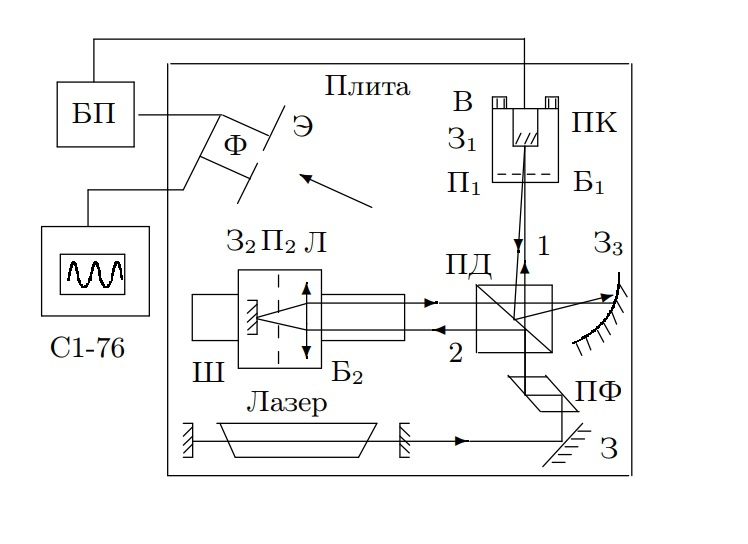
\includegraphics[width=1\textwidth]{set}
    \caption{Схема установки}
    \label{fig:set}
\end{figure}


    Для получения интерференционной картины используется интерферометр Майкельсона, смонтированный на вертикально стоящей металлической плите. Источник света - гелий-неоновый лазер. 
Луч лазера отражается от зеркала З и проходит призму полного внутреннего отражения ПФ, на выходе из которой он имеет поляризацию, близкую к круговой. Далее луч света делится диагональной плоскостью
ПД на два луча.

Луч 1 проходит поляроид П1, отражается под небольшим углом от зеркала З1, снова проходит поляроид П1, и, частично отражаясь от диагональной плоскости делительной призмы, выходит из интерферометра.
Зеркало З1 наклеено на пьезокерамику ПК, которая может осуществлять малые колебания. Поляроид и зеркало с пьзеокерамикой собраны в единой блок ББ1, который крепится к вертикально стоящей плите.
В блоке Б1 имеются юстировочные винты В, которые позволяют регулировать угол наклона зеркала З1. В установке предусмотрена возможность вращения поляроида П1 вокруг луча 1. Угол поворота
отсчитывается по шкале, нанесенной на оправу поляроида.

Луч 2 проходит линзу Л, поляроид П2, отражается от зекрала З2, снова П2, линзу Л и частично выводится делительной призмой из интерферометра. Зеркало З2 установлено в фокальной плоскости линзы
Л. Это сделано для того, чтобы падающий и выходящий лучи всегда были параллельны друг другу. Линза Л, поляроид П2 и зеркало З2 собраны в блок Б2. Этот блок может перемещаться вдодь штанги Ш,
жестко связанной с плитой интерферометра. Длина штанги 90 см. В установке предусмотрена возможность небольшого перемещения блока Б2 перпендикулярно лучу, что позволяет регулировать расстояние между
падающим и выходящим из блока лучами. При измерениях блок Б2 крепится к штанге при помощи двух винтов. Вдоль штанги нанесены деления через один см. При перемещении блока Б2 на L, разность хода 
между лучами 1 и 2 изменяется на 2L.

Лучи 1 и 2 накладываются друг на друга и интерферируют вблизи задней грани делительной призмы ПД. Сферическое зеркало Зз с небольшим фокусным расстоянием увеличивает картину. Интенсивность света
регистрируется фотодиодом Ф. Сигнал с него усиливается и подается на вход осциллографу.

\section{Теория}

\subsection*{Гелий-неоновый лазер}
Лазер представляет собой интерферометр Фабри-Перо -- газовую трубку с двумя параллельными зеркалами по обе стороны. В лазере длиной $L$ для излучения вдоль оси для резонансных частот выполняется
\begin{equation}
f_m = \dfrac{c}{\lambda_m} = \dfrac{mc}{2L}.
\end{equation}
Условие генерации может выполняться для сразу нескольких колебаний с частостами $f_m$, разположенными в диапазоне генерации $2\Delta F$. В этом случае генерируется несколько волн -- \textit{мод} -- межмодовое расстояние для которых
\begin{equation}
\Delta \nu = f_{m+1} - f_m = \dfrac{c}{2L}.
\end{equation}
Число мод можно оценить как 
\begin{equation}
N \approx 1 + \dfrac{2\Delta F}{\Delta \nu}.
\end{equation}
\subsection*{Видимость}
Видимость интерфереционной картины -- параметр, определяемый формулой
\begin{equation}
\gamma = \dfrac{I_{max} - I_{min}}{I_{max} + I_{min}},
\end{equation}
где $I_{max}$, $I_{min}$ -- максимальная и минимальная интенсивности света интерфереционной картины вблизи выбранной точки. Разобьём его на произведение функций параметров установки
$$
\gamma = \gamma_1 \gamma_2 \gamma_3.
$$
Здесь $\gamma_1$ отвечает за соотношение интенсивности интерферирующих волн:
\begin{equation}
\gamma_1 = \dfrac{2\sqrt{\delta}}{1+\delta},
\end{equation}
где $\delta = \frac{B_m^2}{A_m^2}$, $A_m$ и $B_m$ -- амплитуды волн. Параметр $\delta$ определяется устройством разделения волн.\\
Функция $\gamma_2$ отвечает за влияние разности хода и спектрального состава волн,
$$
\gamma_2 = \dfrac{\sum\limits_n A^2_n \cos \frac{2\pi \Delta \nu n l}{c}}{\sum\limits_n A_n^2},
$$
где $l$ -- разность хода, $\Delta \nu$ -- спектральный состав излучения, $A_n^2$ -- интенсивности мод. В непрерывном пределе получим
$$
\gamma_2 = e^{-\left(\frac{\pi \Delta F l}{c}\right)^2}
$$
-- для гауссова линии излучения с полушириной $\Delta F$ получили гауссову зависимость $\gamma_2 = \gamma_2(l)$ с полушириной 
\begin{equation}
l_{1/2} = \dfrac{c}{\pi \Delta F}\sqrt{\ln 2} \approx \dfrac{0.26 c}{\Delta F}.
\end{equation}
Последняя функция $\gamma_3$ отвечает за разность в поляризации. Если $\alpha$ -- угол между плоскостями поляризаций волн, то
\begin{equation}
\gamma_3 = |\cos \alpha|.
\end{equation}

\section{Ход работы и обработка}

По картине на экране осциллографа можно определить параметры видимости по следующим формулам:
\begin{equation}
\delta = \dfrac{h_1}{h_2},
\end{equation}
\begin{equation}
\gamma = \dfrac{h_4 - h_3}{h_4 + h_3},
\end{equation}
Здесь 0 -- уровень при отсутствии лучей, 1 и 2 -- при закрытии одного из них. Используя $\delta$, можно рассчитать $\gamma_1$ по формуле (5).\\ 
При условии одинаковой поляризации лучей ($\alpha = 0$),
\begin{equation}
\gamma_2 = \dfrac{\gamma}{\gamma_1}.
\end{equation}
Если же разность хода отсутствует ($l = 0$), то
\begin{equation}
\gamma_3 = \dfrac{\gamma}{\gamma_1}.
\end{equation}
Исследуем зависимость видности интерференционной картины от угла поворота поляроида П1 при нулевой разности хода. Рассчитаем величины и занесем всё в таблицу:

\begin{table}[H]
	\centering
	\begin{tabular}{|c|c|c|c|c|c|c|c|}
	\hline
	\textbf{Градусов} & \textbf{60}  & \textbf{50} & \textbf{40}  & \textbf{30}  & \textbf{20}  & \textbf{10}  & \textbf{0}   \\ \hline
	h1                & 10           & 15          & 25           & 25           & 30           & 30           & 25           \\ \hline
	h2                & 220          & 220         & 225          & 220          & 220          & 225          & 225          \\ \hline
	h3                & 170          & 160         & 150          & 150          & 160          & 170          & 180          \\ \hline
	h4                & 290          & 310         & 350          & 340          & 350          & 335          & 320          \\ \hline
	$\gamma$          & 0,261        & 0,319       & 0,400        & 0,388        & 0,373        & 0,327        & 0,280        \\ \hline
	$\delta$          & 0,045        & 0,068       & 0,111        & 0,114        & 0,136        & 0,133        & 0,111        \\ \hline
	$\gamma_2$        & 0,408        & 0,489       & 0,600        & 0,605        & 0,650        & 0,644        & 0,600        \\ \hline
	$\gamma_3$        & 0,640        & 0,653       & 0,667        & 0,640        & 0,573        & 0,507        & 0,467        \\ \hline
	\textbf{Градусов} & \textbf{100} & \textbf{45} & \textbf{180} & \textbf{170} & \textbf{160} & \textbf{150} & \textbf{130} \\ \hline
	h1                & 5            & 30          & 10           & 10           & 5            & 5            & 0            \\ \hline
	h2                & 230          & 240         & 240          & 240          & 245          & 240          & 245          \\ \hline
	h3                & 220          & 165         & 200          & 210          & 220          & 225          & 235          \\ \hline
	h4                & 260          & 365         & 300          & 290          & 280          & 270          & 260          \\ \hline
	$\gamma$          & 0,083        & 0,377       & 0,200        & 0,160        & 0,120        & 0,091        & 0,051        \\ \hline
	$\delta$          & 0,022        & 0,125       & 0,042        & 0,042        & 0,020        & 0,021        & 0,000        \\ \hline
	$\gamma_2$        & 0,289        & 0,629       & 0,392        & 0,392        & 0,280        & 0,283        & 0,000        \\ \hline
	$\gamma_3$        & 0,289        & 0,600       & 0,510        & 0,408        & 0,429        & 0,321        &              \\ \hline
	\end{tabular}
	\caption{Данные}
	\label{tab:data}
\end{table}
Построим по этим данным график $\gamma_3(\alpha)$ и убедимся, что зависимость действительно от косинуса:

\begin{figure}[H]
    \centering
    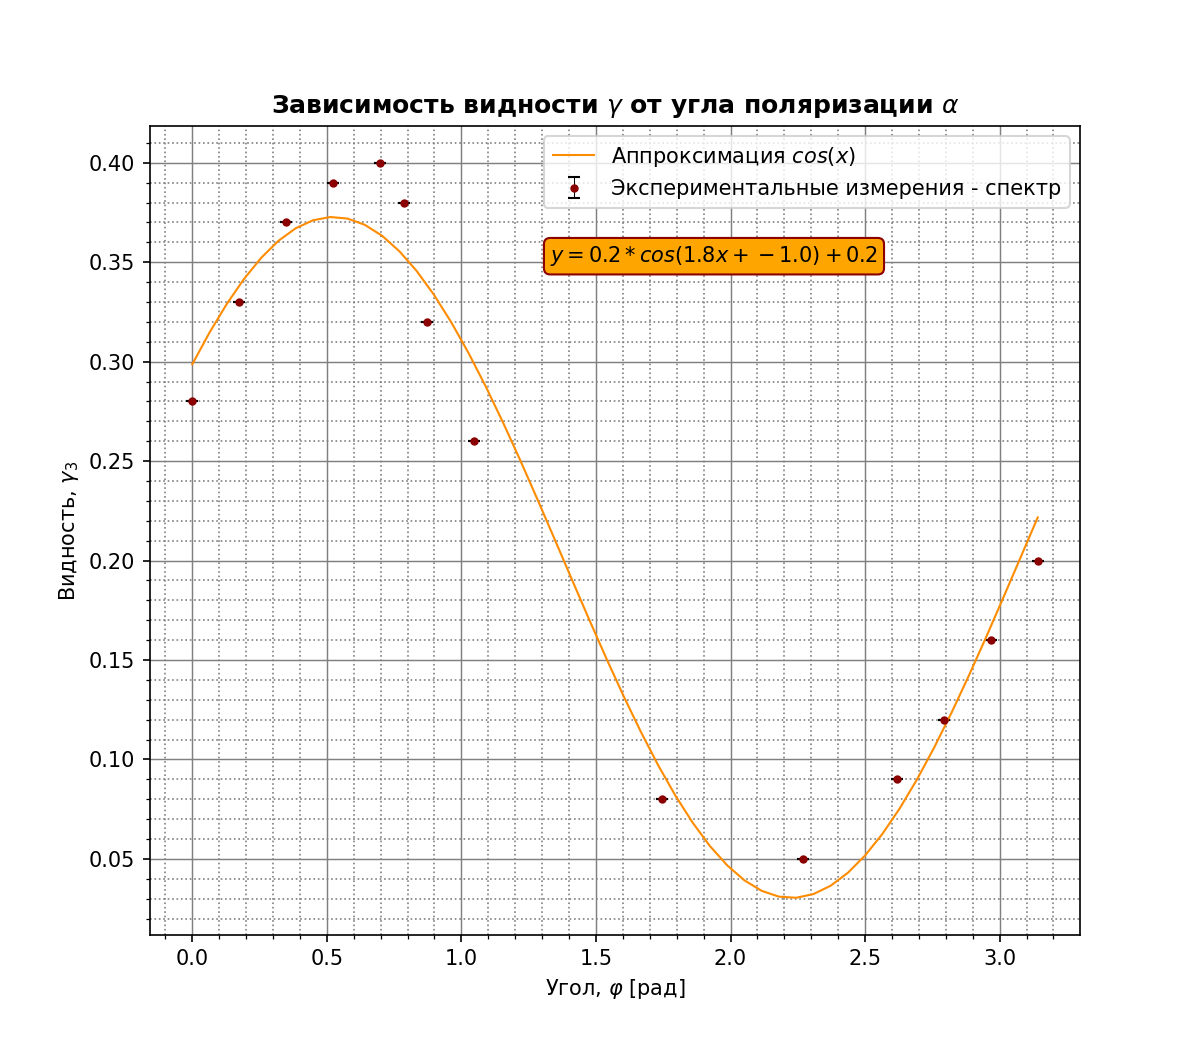
\includegraphics[width=0.85\textwidth]{plot4--5--2-3.png}
    \label{fig:plot1}
\end{figure}
Исследуем зависимость видности от разности хода. Для этого установим поляроид П1 в положение, в котором картина видна наиболее четко. Снимем зависимость h1, h2, h3, h4 от координаты блока Б2.
Занесем результаты в таблицу.

\begin{table}[H]
	\centering
	\begin{tabular}{|c|c|c|c|c|c|c|c|c|c|c|}
	\hline
	\textbf{см}         & \textbf{17} & \textbf{20} & \textbf{22} & \textbf{24} & \textbf{26} & \textbf{28} & \textbf{30} & \textbf{32} & \textbf{34} & \textbf{36} \\ \hline
	\textbf{h1}         & 60          & 35          & 20          & 125         & 30          & 140         & 110         & 90          & 110         & 135         \\ \hline
	\textbf{h2}         & 120         & 185         & 100         & 120         & 210         & 140         & 205         & 170         & 270         & 210         \\ \hline
	\textbf{h3}         & 130         & 260         & 70          & 200         & 215         & 260         & 300         & 250         & 380         & 330         \\ \hline
	\textbf{h4}         & 215         & 300         & 160         & 240         & 225         & 280         & 320         & 270         & 385         & 340         \\ \hline
	\textbf{$\delta$}   & 0,500       & 0,189       & 0,200       & 1,042       & 0,143       & 1,000       & 0,537       & 0,529       & 0,407       & 0,643       \\ \hline
	\textbf{$\gamma_1$} & 0,943       & 0,732       & 0,745       & 1,000       & 0,661       & 1,000       & 0,953       & 0,951       & 0,907       & 0,976       \\ \hline
	\textbf{$\gamma$}   & 0,246       & 0,071       & 0,391       & 0,091       & 0,023       & 0,037       & 0,032       & 0,038       & 0,007       & 0,015       \\ \hline
	\textbf{$\gamma_2$} & 0,261       & 0,098       & 0,525       & 0,091       & 0,034       & 0,037       & 0,034       & 0,040       & 0,007       & 0,015       \\ \hline
	\textbf{см}         & \textbf{38} & \textbf{40} & \textbf{42} & \textbf{44} & \textbf{46} & \textbf{58} & \textbf{60} & \textbf{62} & \textbf{64} & \textbf{66} \\ \hline
	\textbf{h1}         & 50          & 90          & 90          & 50          & 130         & 20          & 15          & 5           & 20          & 100         \\ \hline
	\textbf{h2}         & 185         & 35          & 120         & 130         & 30          & 140         & 40          & 115         & 100         & 125         \\ \hline
	\textbf{h3}         & 220         & 120         & 200         & 170         & 100         & 150         & 50          & 60          & 100         & 115         \\ \hline
	\textbf{h4}         & 235         & 120         & 210         & 175         & 115         & 160         & 70          & 75          & 125         & 140         \\ \hline
	\textbf{$\delta$}   & 0,270       & 2,571       & 0,750       & 0,385       & 4,333       & 0,143       & 0,375       & 0,043       & 0,200       & 0,800       \\ \hline
	\textbf{$\gamma_1$} & 0,819       & 0,898       & 0,990       & 0,896       & 0,781       & 0,661       & 0,891       & 0,400       & 0,745       & 0,994       \\ \hline
	\textbf{$\gamma$}   & 0,033       & 0,000       & 0,024       & 0,014       & 0,070       & 0,032       & 0,167       & 0,111       & 0,111       & 0,098       \\ \hline
	\textbf{$\gamma_2$} & 0,040       & 0,000       & 0,025       & 0,016       & 0,089       & 0,049       & 0,187       & 0,278       & 0,149       & 0,099       \\ \hline
	\textbf{см}         & \textbf{68} & \textbf{70} & \textbf{72} & \textbf{74} & \textbf{76} & \textbf{78} & \textbf{80} & \textbf{82} & \textbf{84} & \textbf{86} \\ \hline
	\textbf{h1}         & 35          & 20          & 10          & 10          & 110         & 30          & 30          & 20          & 50          & 60          \\ \hline
	\textbf{h2}         & 35          & 65          & 45          & 110         & 60          & 45          & 60          & 75          & 100         & 50          \\ \hline
	\textbf{h3}         & 110         & 70          & 40          & 90          & 50          & 35          & 40          & 60          & 90          & 70          \\ \hline
	\textbf{h4}         & 135         & 100         & 65          & 145         & 100         & 110         & 130         & 135         & 190         & 135         \\ \hline
	\textbf{$\delta$}   & 1,000       & 0,308       & 0,222       & 0,091       & 1,833       & 0,667       & 0,500       & 0,267       & 0,500       & 1,200       \\ \hline
	\textbf{$\gamma_1$} & 1,000       & 0,848       & 0,771       & 0,553       & 0,956       & 0,980       & 0,943       & 0,815       & 0,943       & 0,996       \\ \hline
	\textbf{$\gamma$}   & 0,102       & 0,176       & 0,238       & 0,234       & 0,333       & 0,517       & 0,529       & 0,385       & 0,357       & 0,317       \\ \hline
	\textbf{$\gamma_2$} & 0,102       & 0,208       & 0,309       & 0,423       & 0,349       & 0,528       & 0,562       & 0,472       & 0,379       & 0,318       \\ \hline
	\end{tabular}
	\caption{Данные и результаты}
	\label{tab:data2}
\end{table}
Построим график видности $\gamma_2$ от координаты
\begin{figure}[H]
    \centering
    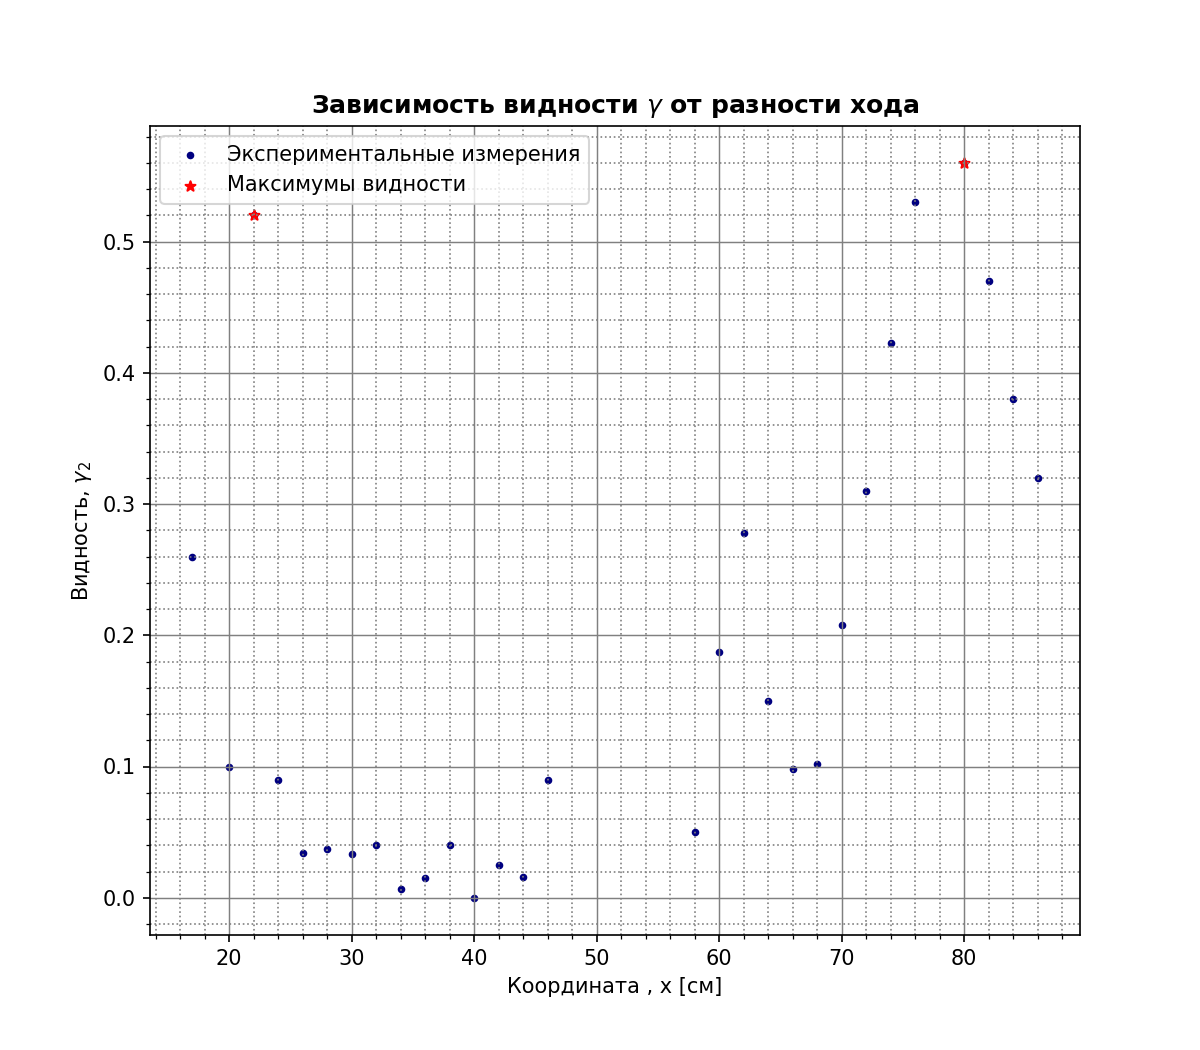
\includegraphics[width=1\textwidth]{plot4--5--2-2.png}
    \label{fig:plot2}
\end{figure}
По расстоянию между максимумами оценим расстояние L между зеркалами:
\begin{equation*}
	L = \frac{\Delta x}{2} = \frac{80 - 22}{2} \text{ см} = 29 \text{ см}
\end{equation*}
Тогда
\begin{equation*}
	\Delta \nu = \frac{c}{2L} = 0,52 \text{ ГГц}
\end{equation*}
Так же можем найти
\begin{equation*}
	\Delta F = \frac{0.26c}{l_{1/2}} = 0,78 \text{ ГГц}
\end{equation*}
\end{document}